\section{Analisi del Server}\label{sec:serveranalisys}


Il server rappresenta l'interfaccia messa a disposizione dal sistema
per lo smistamento e la gestione delle richieste proveniente da parte
dei pazienti e dagli amministratori. La gestione del server è facilitata
da un interfaccia grafica come da Figura \vref{fig:uiservermain}\subref{fig:UIServer}:

\begin{figure}[!b]
 \centering
   \subfloat[][\emph{UIServer}.]{\label{fig:UIServer}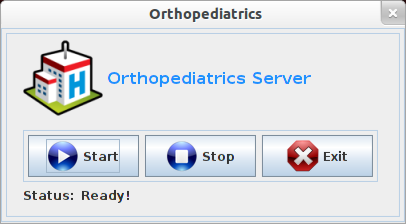
\includegraphics[scale=0.5]{GUI/UIServer}}\\
   \subfloat[][\emph{UIServer Statechart Diagram}.]{\label{fig:uiserverstatechartdiagram}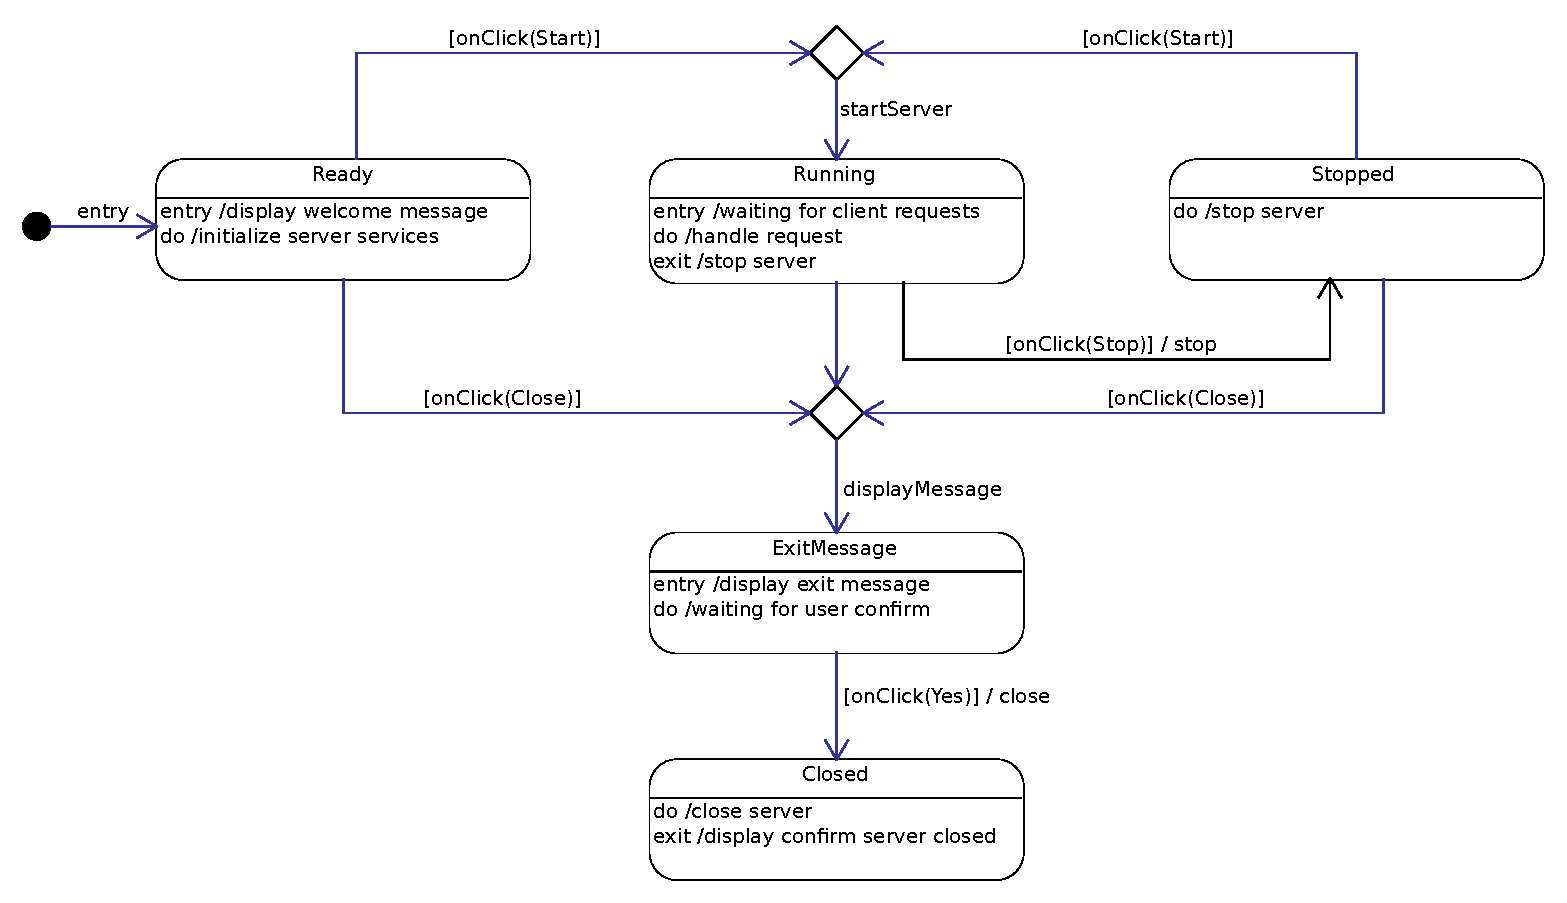
\includegraphics[scale=0.5]{svgs/UIServer-Statechart-Diagrams}}\\ 
 \caption{\emph{A Server Overview}.}
 \label{fig:uiservermain}
\end{figure}



Il server può trovarsi in tre stati diversi, che sono visualizzati
dalla label {}``\emph{Status}'':

\begin{description}
\item[ready] questo stato si ha nel momento in cui viene visualizzato
l'interfaccia grafica (avvio del server)

\item[running] rappresenta lo stato che si raggiunge cliccando
sul bottone {}``Start''

\item[stopped] il server viene messo in pausa e non viene gestita
nessun tipo di richiesta
\end{description}

Cliccando sul pulsante \textbf{Exit} il server termina. Questa descrizione può
essere sintetizzata mediante il diagramma degli stati illustrato in Figura
\vref{fig:uiservermain}\subref{fig:uiserverstatechartdiagram}.


